\section{Pytheas System Architecture}
\label{sec:pytheas:system}

%Having an algorithmic framework of MAB is half of the story.
%To run the logic for per-group control and session grouping at scale, we seek a system design that meets three goals:
Given the algorithmic pieces from the previous section, next 
we discuss how we map them into a system architecture.
  At  a high level, the \mab logic of each group is independently run by frontend clusters,
while the session-to-group mapping is continuously updated by the 
backend.

%\vyas{i dont get any sense of what to expect in this section}

\subsection{Requirements} 
 The \name system design must meet four goals:
\begin{packedenumerate}
\item {\em Fresh data:} The per-group \mab logic should be updated every second with newest QoE measurements.
\item {\em Global scale:} It should handle millions of geo-distributed sessions per second.
\item {\em Responsiveness:} It should respond to requests for decisions from sessions within
 a few  milliseconds.
\item {\em Fault tolerance:} QoE should not be significantly impacted when parts of the system fail.
\end{packedenumerate}

%\tightsubsection{Split control vs. \idea}

%\vyas{dont start with this .. no one knows what split control is!!}
%\vyas{as written it sounds more incremental wrt C3 than it really is!}
%\vyas{not even sure why 6.1 is necessary. i can just move it to related work}

%It is helpful to understand the architectural benefit of \idea by contrasting
%it with split control.  

A natural starting point to achieve this goals might be to adopt a ``split
control plane'' approach advocated by prior work for prediction-based 
approaches~\cite{c3,cfa}.  At a high level, this split control plane has two parts: (1)
a backend cluster that generates centralized predictions  based on  global but
stale data, and (2) a set of geodistributed frontend servers  that use these predictions
from the backend to make decisions on a per-session basis.  
%In addition,  the clients also run per-session adaptation
%algorithms as fall back strategies.  
This split control architecture  achieves  global  scale and
high responsiveness, but fundamentally sacrifices data freshness.  
%While this
%tradeoff was inevitable in the prediction-oriented abstraction adopted by prior
%work~\cite{c3,cfa}, this violates the requirements of running \mab processes.


 \name  preserves the scale and responsiveness of the split control
approach, but extends  in  two key ways to run  \idea with fresh data. First,
each frontend cluster runs  an active \mab algorithm rather than merely
executing the (stale) prediction decisions as in prior work.  Second, the
frontend clusters now run per-group logic, not per-session logic.  This is
inspired by the insight that sessions in the same group are very likely to be
received by the same frontend cluster.  Thus, \idea could achieve high data
freshness on the session group granularity, while having the same scale and
responsiveness to split control.
Next, we discuss the detailed design of the frontend and backend 
 systems. 
 
%  the dper-session decision execution algorithm 
%he \idea architecture used in \name is similar to split control but with a key
%difference: 

 
%To achieve scalability and responsiveness, split
%control performs per-session control logic at frontend clusters, while using
%the backend cluster to make centralized hint based on the global yet stale
%data.  

\subsection{Per-Group Control by Frontends}
\label{subsec:frontend}


The best case for \idea is when all sessions of the same group are received by
the same frontend cluster.  When this is true, we can run the per-group \mab
logic (Section~\ref{subsec:per-group}) in real time with fresh measurements of
the same group.  In fact, this also is the common case.  To show this, we ran
session-grouping logic (Section~\ref{subsec:grouping}) on 8.5 million video
sessions in a real-world trace, and found around 200 groups each minute. Among these groups, we found that (in
Figure~\ref{fig:fraction-same-frontend}) for 95\% of groups, all sessions are
in the same AS, and for 88\% of groups, all sessions are even in the same AS
{\em and} same city.  Since existing session-to-frontend mappings (e.g., DNS or Anycast-based mechnisms) 
are often based on AS
and geographical location, this means that for most groups, their sessions will
be verly likely to be received in the same frontend clusters.

%This means when a per-group logic receives a decision request, all data it needs are received by the same cluster, so the per-group control logic can be updated with in real time with fresh per-group data.


\begin{figure}[t!]
\centering
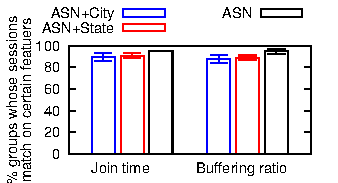
\includegraphics[width=0.45\textwidth]{figures/pytheas-Eval-fraction-same-frontend.pdf}
%\vspace{-0.2cm}
\caption{For most groups, the sessions are in the same ASN and even same city.}
\label{fig:fraction-same-frontend}
\end{figure}

 In practice, however, it is possible that sessions of one group are spread across 
frontend clusters.
%\footnote{We take a pragmatic stance that each session request or
%measurement is directed by one of many geo-distributed frontend clusters via
%DNS or anycast services, like in most today's service providers. Such
%redirection services are usually shared with critical real application traffic,
%so we assume \name does not have control over how a client is redirected to the
%frontend clusters.}
 We have two options in this case:
\begin{packedenumerate}
\item Pick one cluster as the {\em leader} cluster of this group and let it run the \mab logic of the group based on the measurements received by this cluster. Meanwhile, other clusters, called {\em proxy} clusters of the group, simply receive decisions periodically from the leader cluster.
\item Keep the leader cluster and proxy clusters, but let proxy clusters not only receive decisions from the leader, but also forward QoE measurements to the leader cluster.
\end{packedenumerate}
We see a tradeoff between the two options.
While Option 1 is less complex to implement than Option 2, the leader proxy in Option 1 runs per-group logic based on only a subset of sessions, especially when the sessions of a group are evenly spread across many frontend clusters.
We pick Option 2, because it is cleaner in that the per-group logic is based on all sessions in a group. In fact, implementing Option 2 does not add much complexity.
Finally, Option 2 can easily fall back to Option 1 by stop forwarding measurements from proxy clusters to the leader cluster.





\subsection{Updating Session Groups in the Backend}
\label{subsec:backend}

%The role of the backend in group-based control is two-fold.
The backend cluster uses a global, stale view of measurements to update two tables, which are sent
 to the frontend to regroup sessions.
\begin{packeditemize}
\item First, the backend runs the session-grouping logic (Section~\ref{subsec:grouping}) to decide which group each session belongs to, and outputs a {\em session-to-group table}.
\item Second, it decides which frontend should be the leader cluster of each group and outputs a {\em group-to-leader table}. For each group, we select the frontend cluster that receives most sessions in the group as the leader.
\end{packeditemize}
%For each group, we select the frontend cluster that receives most sessions in the group, because this will minimize the number of sessions in the proxy clusters, whose decisions and measurements need to be shared across frontend clusters.
%To this end, each frontend cluster will count the number of sessions each group receives, and sends these counts to the backend.
The backend periodically (by default, every ten minutes) updates the frontend clusters with these two maps.  
%\cameraremove{The only exception when the maps are updated in
%near real time is when flash crowd happens, which will be discussed in the next
%section.}
The only exception for the maps to be updated in
near real time is when one or more frontend clusters fail, which we discuss next.



%\cameraremove{
%\tightsubsection{Handling flash crowds}
%\label{subsec:flashcrowd}
%}
%
%\cameraremove{
%Session groups tend to change slowly, except when flash crowd happens.
%Unlike other grouping drifts, flash crowds do not occur gradually, so the backend needs to react to flash crowds swiftly by regrouping sessions.
%For instance, in Example C (\Section\ref{subsec:limitations}), the flash crowd on a particular object should be grouped together and receive different decisions than others. 
%Fortunately, flash crowds can be detected based on workload and once they are detected, we can simply create a group for these sessions. 
%This is simpler than QoE-based session-grouping logic (\Section\ref{subsec:grouping}), so it can run on a much finer timescale (by default, we run it every 5 seconds).
%For instance, in video streaming, \name can detect a flash crowd by monitoring how many sessions are watching each video object (through simple streaming algorithms~\cite{alon1996space}), and react by creating a new group for this particular object.
%
%Inspired by this observation, \name handles flash crowds by a ``fast channel'' between frontend and backend, where each frontend cluster frequently updates the backend with basic statistics of workload (e.g., number of video sessions watching each object), and the backend runs  a simple algorithm to detect flash crowds (e.g., look for any sudden increase in the population of an object), and creates new groups accordingly.
%This fast channel provides an opportunity to handle grouping drifts (such as frontend failure discussed in the next section) that happen frequently but can be detected with algorithms.
%}


\subsection{Fault Tolerance}
\label{subsec:fault}
 As we rely on fault-tolerant components for
 the  individual components of \name within each cluster (see Section~\ref{sec:pytheas:impl}), 
the residual failure mode of \name is when some clusters are not available.
 Next, we discuss how we tackle three potential concerns in this setting.

First, if a failed frontend is the leader cluster of a group, the states of the \mab logic of the group will be lost, and we will not be able to update decisions for sessions of the group.
To detect frontend failures and minimize their impact, each frontend sends frequent heartbeat messages through a ``fast channel'' every few seconds (by default, every five seconds) to the backend, so backend can detect frontend failures based on these heartbeat messages.
%\cameraremove{To minimize the impact, the backend detects frontend failures based on the workload update sent by the fast channel (\Section\ref{subsec:flashcrowd}), which is updated frequently (by default, every 5 seconds).}
Once the backend detects a frontend failure, it will select a new leader clusters for any group whose leader cluster has been the failed one,
and recover the per-group logic in the new leader cluster.
To recover the per-group states,  each leader always shares the per-group states with its proxy clusters in the decision update messages, so that when a proxy cluster is selected as the new leader, it can recover the per-group states as they are cached locally.
Note that even without a leader cluster, a proxy cluster can still respond requests with the cached decisions made by the leader cluster before it fails.


Second, the sessions who are assigned to the failed frontend will not  receive control decisions.
To minimize this impact, \name will fall back to the native control logic.
Take video streaming as an example, when \name is not available, the client-side video player can fall back to the control logic built into the client-side application (e.g., local bitrate adaptation) to achieve graceful QoE degradation, rather than crash~\cite{c3}.

Finally, if the backend cluster is not available, \name will not be able to update groups.
However, \name does not rely on backend to makde decisions, so clients will still receive (albeit suboptimal) decisions made by \name's frontend clusters. %the frontend clusters can still run per-group control logic, receive measurement data, and respond to decision requests.

%\newpage






